\chapter{タイピングゲームの設計と実装}\chaplab{conclusion}
この節ではタイピングゲームの設計と実装に関して説明する.

\subsection{タイピングゲームの設計}
タイピングゲームは図4.1のように表示され,ユーザは表示されている英単語を入力していく.ユーザが任意のキーを入力したときにゲームが開始され,それと同時にタイピングゲームにかかる時間の計測が始まる.英単語は既に入力し終わっている文字を灰色,スペリングを誤った文字を赤色,まだ入力していない文字を黒で示している.1つの英単語を入力し終わるごとに新たな単語が表示される.100単語タイプし終わるとゲームクリアとなる.スコアはスペリングを誤るたびに10点減点され,100問タイプし終わった時間が速いほど加点される.プレイに応じてユーザの現在のタイムやスコアも表示される.ユーザがタイピングゲームを行った中で最も高いスコアはハイスコアとして表示される.またスペリングを誤ったときや英単語を1単語入力し終わる度に効果音が鳴る.

\subsection{タイピングゲームの実装}
「初めて学ぶ人のためのJavaScript入門:タイピングゲームを作る」\footnote{\url{http://www.pori2.net/js/key/3.html}}を参考にしてタイピングゲームの実装を行った.サイトではユーザのキーコードの入力を受けてその入力が表示されているアルファベットと一致しているかどうかを判定し,ユーザがアルファベットを200文字正しく入力するまでの時間を計るアルゴリズムを示すソースコードが書かれている.本研究ではそのコードを以下のように改変・追加することで,研究のためのタイピングゲームの実装を行った.

まずユーザに入力させていたアルファベットを英単語に変更した.
次にユーザが正しく英単語を入力したときは正解を示す効果音,スペリング誤りをしたときは不正解を示す効果音が鳴る機能を実装した.またユーザが英単語をタイプしているとき,スペリングを誤った文字を赤く,既に入力し終わっている文字を灰色で表示させるように実装を行った.

またタイピングゲームにゲーム的な要素を取り入れるため,ユーザがタイピングゲームを行うのにかかった時間とともにタイピングの正確さや速さを元に算出したスコアを表示させるようにした.スコアはゲームが終了するまでの時間が短いほど,ユーザがスペリング誤りをした回数が少ないほど高くなるように設定した.

最後にユーザが英単語を1単語入力し終わる度にユーザが実際に入力したアルファベットの文字列とそのときタイピングゲーム上で表示していた英単語,ユーザが英単語を入力するのにかかった時間をサーバに送るように実装を行った.

本研究ではタイピングを行ったときに鳴る効果音はウェブサイト\footnote{\url{http://musicisvfr.com/free/se/quiz01.html}}で公開されているものを使用している.使用に関してはCreative Commonsライセンス\footnote{\url{http://creativecommons.org/licenses/by/4.0/deed.ja}}に基づいて素材の改変が可能なものを使用している.

タイピングゲームでタイプする英単語としてベーシック英語\cite{simpleenglish}を用いた.これは言語学者のチャールズ・ケイ・オグデンによって考案された英語の体系で,基本単語850語リストは英語の初級者向け語彙として使われており,このうち冠詞aなどを取り除いた842語をタイピングゲームの問題にすることから,タイピングゲームを行うことによって英語学習にも役立つ可能性があると考えられる.ユーザが打ち込むベーシック英語の英単語とその訳語はウェブサイト\footnote{\url{http://www.catch.jp/wiki/index.php?english\%2F800_Basic_English}}で公開されているものを使用している.

\begin{figure*}[t]
	\begin{center}
		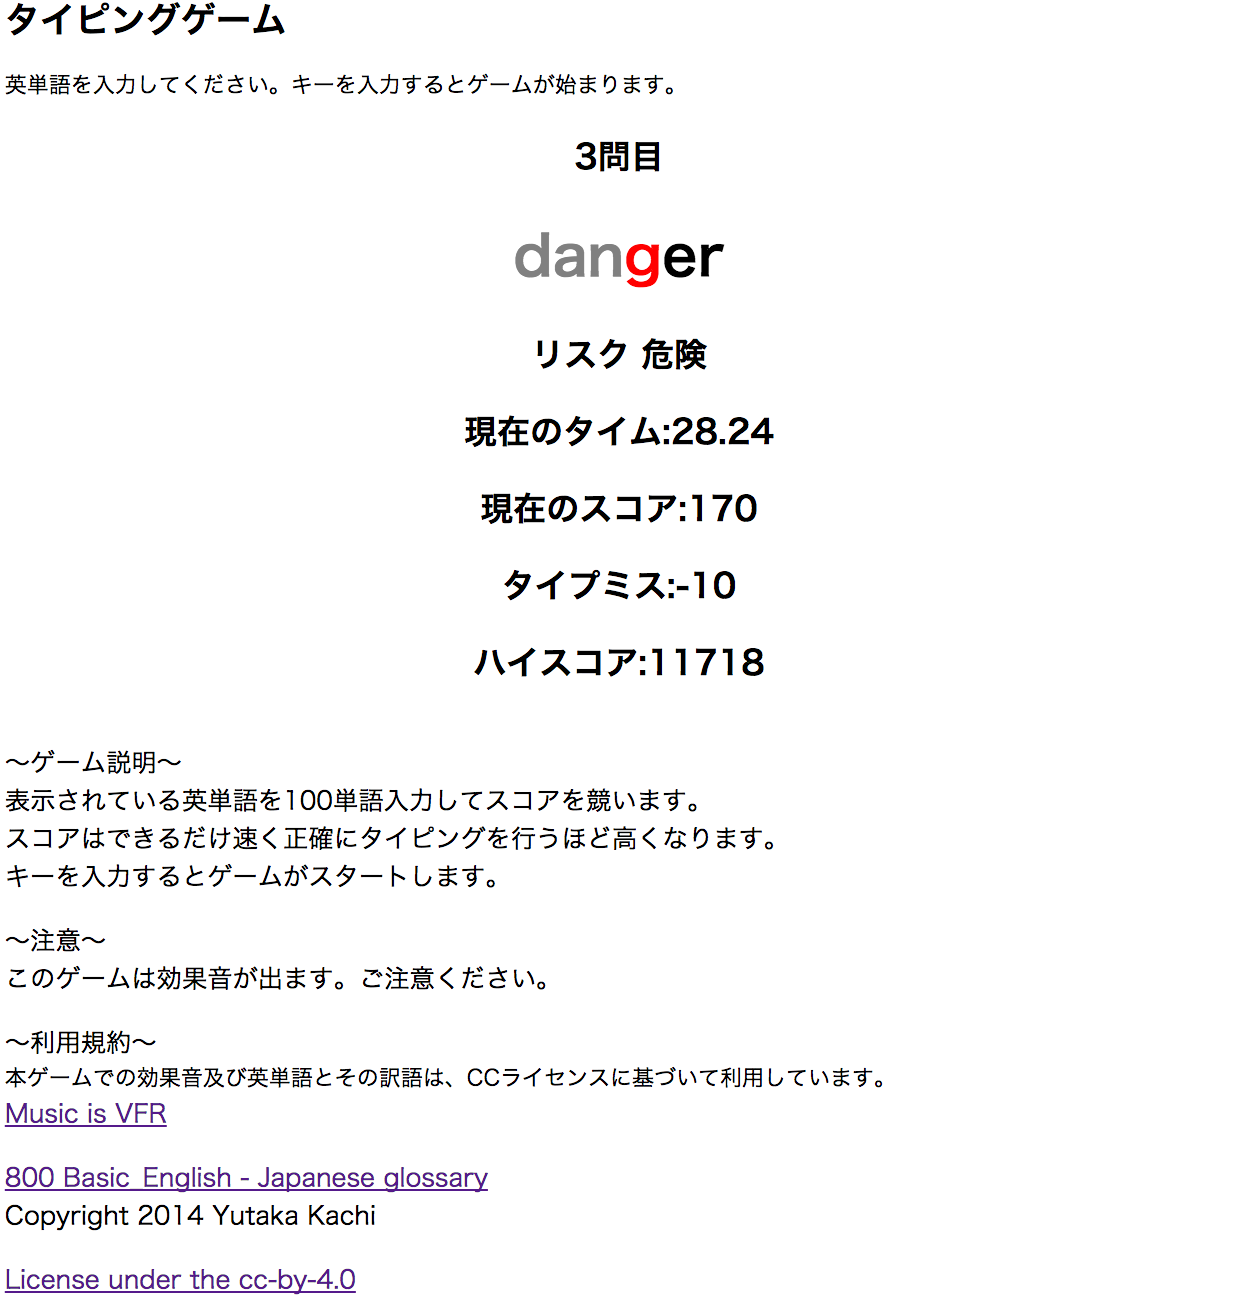
\includegraphics[width=15cm]{typing_game2.png}
		\caption{タイピングゲームのスクリーンショット}
		\label{LabelExa}
	\end{center}
\end{figure*}